\documentclass[a4paper,12pt,english, T1]{book}
\usepackage[utf8]{inputenc}
\usepackage[T1]{fontenc}
\usepackage{tikz-dependency}
\usepackage{times}
\usepackage{multirow}
\usepackage{tablefootnote}
\usepackage{booktabs}
\usepackage{covington}
\usepackage{relsize}
\usepackage{hyperref}
\usepackage{appendix}
\usepackage{duomasterforside}
\usepackage{emptypage}
\usepackage{tocbibind}
\usepackage{url}
\usepackage{tikz}
\usepackage{apacite}
\usepackage{amsmath}

% for quotations
\usepackage{dirtytalk}
\usepackage{csquotes}

% for images
\usepackage{graphicx}
\graphicspath{ {img/} }

\usepackage{fancyhdr}
\pagestyle{fancy}
\fancyhf{}
\renewcommand{\sectionmark}[1]{\markright{\thesection.\ #1}}
\renewcommand{\chaptermark}[1]{\markboth{\textsc{\thechapter.\ #1}}{}}
\lhead[\leftmark]{}
\rhead[]{\rightmark}
\lfoot[\thepage]{}
\rfoot[]{\thepage}

\title{Improving Semantic Frame Accuracy for Semantic Dependency Parsing}
\author{Arash Saidi}

\begin{document}
\newcommand\tab[1][1cm]{\hspace*{#1}}
\duoforside{}

\chapter*{Abstract}
\thispagestyle{empty}

This thesis presents an in-depth contrastive error analysis of a set of semantic dependency parsing systems. Based on the empirical results of our analysis we found semantic frame classification to be an interesting case study. As part of this thesis we have made a semantic frame classifier that outperforms previous results. The semantic frame classifier is the result of rigorous experimentation with four set of features: (1) lexical, (2) morphological, (3) syntactic, and (4) semantic. We show that our results outperform previous results. We also show that our classifier can be used to extend and improve the frame semantic classification accuracy of two existing state-of-the-art semantic dependency parsing systems.

% the results of frame classification of two existing state-of-the-art semantic dependency parsing systems.

% This thesis presents a systematic, empirical investigation of how an existing PoS tag set can be modified and optimized for the task of syntactic dependency parsing of Norwegian. The tag set of the Norwegian Dependency Treebank is modified and optimized through experiments with the morphological features in the treebank. The experiments are complemented by evaluation of a range of state-of- the-art PoS taggers and syntactic parsers applied to Norwegian. The results of our work are concrete contributions to the Norwegian NLP community: (i) a data set split (training/development/test) of the Norwegian Dependency Treebank; (ii) a PoS tag set optimized for syntactic dependency parsing of Norwegian; (iii) a PoS tagger model trained on the treebank; and (iv) a syntactic parser model trained on the treebank.
\chapter*{Acknowledgements}
\thispagestyle{empty}

This thesis is submitted for the degree of Master of Science at the University of Oslo. My supervisors have been Stephan Oepen and Lilja Øvrelid. I am thankful for their insights, helpful advice and patience.

I want to thank my good friend, fellow student, and co-worker Petter Hohle for proofreading and being a great motivator. I want to thank my co-worker Anna Therese Hägg for proofreading. I thank my girlfriend Marit for encouragement, love and support.

\frontmatter{}
\fancyhead[LE]{\nouppercase\leftmark}
\fancyhead[RO]{\nouppercase\rightmark}
\tableofcontents{}
\listoftables{}
\listoffigures{}

\mainmatter{}
\chapter{Introduction}
\label{chap:introduction}

% Motivere hva som er resultatet, hva har jeg gjort, og hvem som trenger det, hvilken spørsmål har du stilt.

Semantic dependency parsing is a Natural Language Processing (NLP) task that aims at producing meaning representations at the sentence-level. We can state the aims of semantic dependency parsing as a way of expressing predicate-argument relations in order to answer the question of \textit{Who did What to Whom?} In this regard there is certainly an overlap between semantic dependency parsing  and \textit{semantic role labeling} (SRL). 

The task of SRL is concerned with detecting the arguments of a predicate in a given sentence. Semantic dependency parsing usually has a broader scope than argument detection. In addition to the goals of SRL, semantic dependency parsing attempts to identify various semantic phenomena, such as negation, topicalization, relative clauses, and other scopal dependencies that are not part of the scope of SRL.

Examining the research community and the publications in the field of dependency parsing, we can see a growing interest in semantic dependency parsing in recent years. This can be attributed to both the advances made in the accuracy of state-of-the-art parsers, but also due to the successful application of such parsers and their representations in a wide range of computational tasks such as Information Extraction, Textual Inference, Machine Translation, Semantic Search, and Sentiment Analysis. A set of so-called shared tasks on semantic dependency parsing, which we will present in this thesis, have also stimulated the research community towards more research on this specific type of dependency parsing.

In this thesis we present our contribution to the field of semantic dependency parsing by doing a high-level contrastive error analysis of various state-of-the-art semantic dependency parsing systems. We will closely examine their results, and compare them in order to gain insights into the areas with the potential of improvements in parsing accuracy. We will show that the error analysis provided us with the grounds for examining the so-called frames, also referred to as sense distinctions, in order to make an attempt at improving previous results. Based on this analysis we build our own pipeline for classifying semantic frames. These frames are added as an extra layer to the graph annotations of semantic dependencies. So in this sense they are not part of the semantic dependency graph itself, but acts as additional semantic information. The classification of the frames themselves rely on the semantic dependency graph as features for training the classifier.

\section{Overview} 

% Background
\paragraph{Chapter 2} provides a background for our thesis. In this chapter we briefly outline dependency grammar, and then examine various approaches to dependency based parsing. We differentiate between grammar- and data-driven dependency parsing, and formally describe both of these approaches to dependency parsing. We divide data-driven dependency parsing in two main classes: transition-based and graph-based models. We examine these two models and give examples of their implementation by presenting a few examples of tools that are openly available. Finally, we define semantic dependency parsing, and show how this approach differentiates from syntactic dependency parsing. We will also argue why we should focus on semantic dependency parsing, and provide arguments for the reasoning behind writing this thesis.

\paragraph{Chapter 3} examines a few selected state-of-the-art semantic dependency parsers. We have chosen to focus on a set of data-driven parsers that where part of the Task 18 at SemEval 2015 on \textit{Broad-Coverage Semantic Dependency Parsing} (SemEval-2015) \cite{Oepen:15}. We present the parsing systems that where part of this task, and provide the reader with a background to the technology that drives them. We will also examine the target representations used for training and testing. Here we also examine Task 8 at SemEval 2014 (SemEval-2014) (see \citeA{Oepen:14}, in order to provide the reader with more background to SemEval 2015, and the changes from one year to the next.

\paragraph{Chapter 4} builds on the previous chapter by examining the results submitted by a set of parsing systems to SemEval-2015. By way of an in-depth contrastive error analysis of a set of state-of-the-art parsers we gain insights into some common errors that these parsers share. We examine four factors of semantic dependency parsing: (1) length factors, (2) graph factors, and (3) linguistic factors and (4) frames accuracy. The insights from this chapter lay the empirical foundation for our own classification task.

\paragraph{Chapter 5} examines our own pipeline for classifying semantic frames. The analysis in Chapter \ref{chap:semantic} led us in choosing semantic frames as the focal point of our own work. In this chapter we build a pipeline for classifying semantic frames by examining a set of machine learning algorithms. We start off by presenting a baseline accuracy, and see if we can improve upon this baseline by fine tuning the machine learning algorithms, and by way of exploring a set of features used for training. We show that by using a wide range of features for our classifier, we can achieve state-of-the-art results in predicting semantic frames.

\paragraph{Chapter 6} is a summary and conclusion of our thesis. Here we give a short overview of what we have achieved in our thesis, and discuss how this relates to the research on semantic dependency parsing at large. We also discuss the possibilities for future work that might benefit from the analysis and classification task performed in our thesis.
\chapter{Background}
\label{chap:background}

This chapter provides and introduction to Dependency Grammar and Dependency
Parsing and the technical aspects ranging from the early development to state-of-the-art
dependency parsing techniques. 
\chapter{Semantic Dependency Parsing with Frames}
\label{chap:parsing}
\chapter{In-depth Contrastive Error Analysis}
\label{chap:analysis}

% Length
% Graph factors
% Linguistic factors

% Peking: Ensemble method, combination of transition-based and graph-based
% Turku: Support Vector Machines
% Lisbon: A graph algorithm


In this chapter we present an in-depth contrastive error analysis of the results of SemEval-2015 for the Peking, Turku and Lisbon systems described in Chapter \ref{chap:semantic}. As mentioned in the previous chapter, there where 6 submissions to SemEval-2015, including an `in-official' submission by a sub-set of the task organizers. We have made the choice of focusing on three of these parsing systems in our analysis. This is based on three criteria:

\begin{enumerate}
    \item The chosen systems have the highest overall scores in SemEval-2015.
    \item The technical approach of the three parsing systems are different from one another: both the local transition-based and global graph-based models that we examined in Chapter \ref{chap:background} are represented.
    \item When choosing between submissions where similar technical approach has been used, we exclude the system with the overall lower accuracy score.
\end{enumerate}

The aim of our in-depth contrastive error analysis is to gain insight into the state-of-the-art in semantic dependency parsing. We perform our study in order to:

\begin{enumerate}
    \item Find similarities and differences in the results among a chosen set of parsing systems in order to compare and contrast their strengths and weaknesses.
    \item Empirically identify and verify which types of errors that can be the focus of future research on improving the accuracy of the state-of-the-art in semantic dependency parsing.
    \item Examine whether an ensemble method based on the strengths of different parsing systems is possible in order to improve upon existing systems.
\end{enumerate}

% We will argue that the analysis presented in this chapter can highlight the correlation between the specific types of errors that these parsers make and their theoretical foundation. The analysis presented is thus based on the general knowledge of the parsing systems, as described in Chapter \ref{chap:semantic}, and the specific observations made in our analysis of their results from SemEval-2015.

In our analysis we draw inspiration from three similar studies performed by \citeA{McD:Niv:07}, \citeA{McD:Niv:11}, and \citeA{Choi:Tetreaul:Stent:15}. In these studies a comparative analysis of a set of syntactic parsers is presented where various types of errors are highlighted. The first and second study focus on three types of errors: (1) length factors, (2) graph factors, and (3) linguistic factors. The third study, in addition to these three factors, also examine the speed of parsers. We will structure our analysis in a similar fashion, but exclude speed, and include a fourth type error analysis where we examine the multi-classification task of frame predication.

In addition to narrowing down the scope in terms of choosing three parsing systems, we also exclude results for the PAS target representation. The reasoning behind this is that the DM and PAS target representations are relatively similar. Examining Table \ref{fig:data} in Chapter \ref{chap:semantic}, we observe that DM and PAS are close to identical in the number of labels, percentage of graphs being trees, and percentage of dependencies being projective. The major difference between the two target representations is the percentage of so-called singletons, i.e. nodes outside the graph. The DM target representation has approximately 5 times as many singletons as PAS. With the exception of singletons, we assume that our analysis of the DM results will yield similar results as PAS. This hypothesis was confirmed when running our parts of our analysis on PAS.

However, before we embark on our in-depth contrastive error analysis, we recap overall statistics on the three parsing systems that are the basis for our analysis.

\section{Overall Accuracy}

\begin{table}
    \centering
    \begin{tabular}{@{}cccccccccc@{}}
        \toprule
        \multicolumn{1}{c}{ }
        & \multicolumn{1}{c}{ }
        & \multicolumn{4}{c}{\textbf{DM}}
        & \multicolumn{4}{c}{\textbf{PSD}} \\
        \cmidrule(lr){3-6}
        \cmidrule(lr){7-10}
        &
        LF.av &
        LF & LP & LR & FF &
        LF & LP & LR & FF \\
        \midrule
        Peking & 85.33 & 89.09 & 90.93 & 87.32 & 63.08 & 75.66 & 78.60 & 72.93 & 49.95 \\
        Lisbon & 85.15 & 88.21 & 89.84 & 86.64 & 00.15 & 76.36 & 78.62 & 74.23 & 00.03 \\
        Lisbon* & 86.23 & 89.44 & 90.52 & 88.39 & 00.20 & 77.58 & 79.88 & 75.41 & 00.06 \\
        Turku* & 83.47 & 86.17 & 87.80 & 84.60 & 54.67 & 73.63 & 76.10 & 71.32 & 53.20 \\
        \bottomrule
        
        \\
        \toprule
        \multicolumn{1}{c}{ }
        & \multicolumn{1}{c}{ }
        & \multicolumn{4}{c}{\textbf{DM}}
        & \multicolumn{4}{c}{\textbf{PSD}} \\
        \cmidrule(lr){3-6}
        \cmidrule(lr){7-10}
        &
        LF.av &
        LF & LP & LR & FF &
        LF & LP & LR & FF \\
        \midrule
        Lisbon & 81.15 & 81.75 & 84.81 & 78.90 & 00.27 & 74.82 & 78.68 & 71.31 & 02.09 \\
        Peking & 80.78 & 81.84 & 84.29 & 79.53 & 47.49 & 73.28 & 77.36 & 69.61 & 34.28 \\
        Lisbon* & 82.53 & 83.77 & 85.79 & 81.84 & 00.35 & 76.18 & 80.12 & 72.61 & 02.25 \\
        Turku* & 78.85 & 79.01 & 81.54 & 76.63 & 39.15 & 71.59 & 74.92 & 68.55 & 38.75 \\
        \bottomrule
    \end{tabular}
    \caption{SemEval-2015 results from the open track (marked *) and closed track (unmarked) of the in-domain (top) and out-of-domain (bottom) data for the three parsers included our the analysis.}
    \label{fig:data:recap}
\end{table}

In Chapter \ref{chap:semantic} we reviewed the technical aspects of the three parsing systems we will examine here. The Peking system: an ensemble of transition-based and graph-based models, the Turku system: a combination of several classifiers for specific aspects of the semantic dependency graphs, and the Lisbon system: a graph-based feature-rich linear model that parametrize globally over first and second order dependencies.

In Table \ref{fig:data:recap} we can see the performance of the three parsers. An obvious aspect of the results is that the parsing systems perform better on the in-domain versus the out-of-domain data sets. This is to be expected, as data-driven parsing will perform better on data that resembles the data used for training.

The predictions could be run in an open and closed track, which we described in Chapter \ref{chap:semantic}. Lisbon is the only team that participated in both tracks, Peking in the open and Turku in the closed. 


\section{Length factors}

As \citeA{McD:Niv:07} point out, it is well known that syntactic parsing systems produce results with lower accuracy for longer sentences. We observe the same phenomena in the results from our chosen set of parsers from SemEval-2015. Parsing accuracy is highly correlated with sentence length. \citeA{McD:Niv:11} claim that this is primarily due to more complex constructions in longer sentences, such as prepositions, conjunctions, and multi-class sentences. 

Another type of length factor is the length of dependencies, which also has an impact on the accuracy of predictions. We define the length of a dependency from word $w_i$ to $w_j$ as $j - i$. For the English language, and from examining the data sets used in SemEval-2015, we can generally state that short dependencies are modifiers of nouns, such as determiners, adjectives or pronouns. Longer dependencies are in most cases words that modify the main verb or root of the sentence. 

\subsection{Sentence length}

\subsection{Dependency length}


% conclusion
Both sentence and dependency length have a distribution in the data sets where the frequency of a length factor is correlated with the accuracy for parsing that specific length. The higher the frequency of a given length factor, the more likely that the parsing system has a higher accuracy when parsing a sentence or dependency with a given length. It is therefore important not to exaggerate the importance of the length factor itself, but rather the distribution with which it occurs in the data used for training. So a different data set and distribution would result in, if our assumptions are correct, parsing systems with a different correlation between length and accuracy. 

However, since we are dealing with natural language, we can also assume that a relatively similar distribution of sentence and dependency lengths observed in the SemEval-2015 data sets will be prevalent in other annotated corpora. We will now turn our attention to specific graph factors, such as distance to root, projectivity, and singletons, and examine the accuracy of the three parsing systems in relation to these aspects of semantic dependency parsing.

\section{Graph factors}
% distance to root
% projectivity
% singletons

\section{Linguistic factors}
% part of speech
% labels

\section{Frames}
% just frames
% complete frames

\section{Conclusions}

In this chapter we have examined the results of Peking, Turku and Lisbon parsing systems as submitted to SemEval-2015. Our examinations have uncovered some interesting phenomena, such as the fact that the overall accuracy of all parsing systems drop in correlation to sentence and dependency length. That the parsing systems are more prone to error in regards to certain graph and linguistic factors, and that these are highly correlated with the frequency with which these factors are represented in the data sets.

However, the error analysis did not produce enough evidence to build an overall strategy for improving upon the results of the three semantic dependency parsers examined in this chapter. As mentioned in previously, we have instead chosen to focus on improving the accuracy on the classification task of predicting semantic frames. This aspect of semantic dependency parsing is not well researched, and the results of our analysis seem to indicate that there can be room for improvements on previous research in this area.

% Input for graph images
% \begin{figure}[h]
% \caption{Caption}
% \centering
% 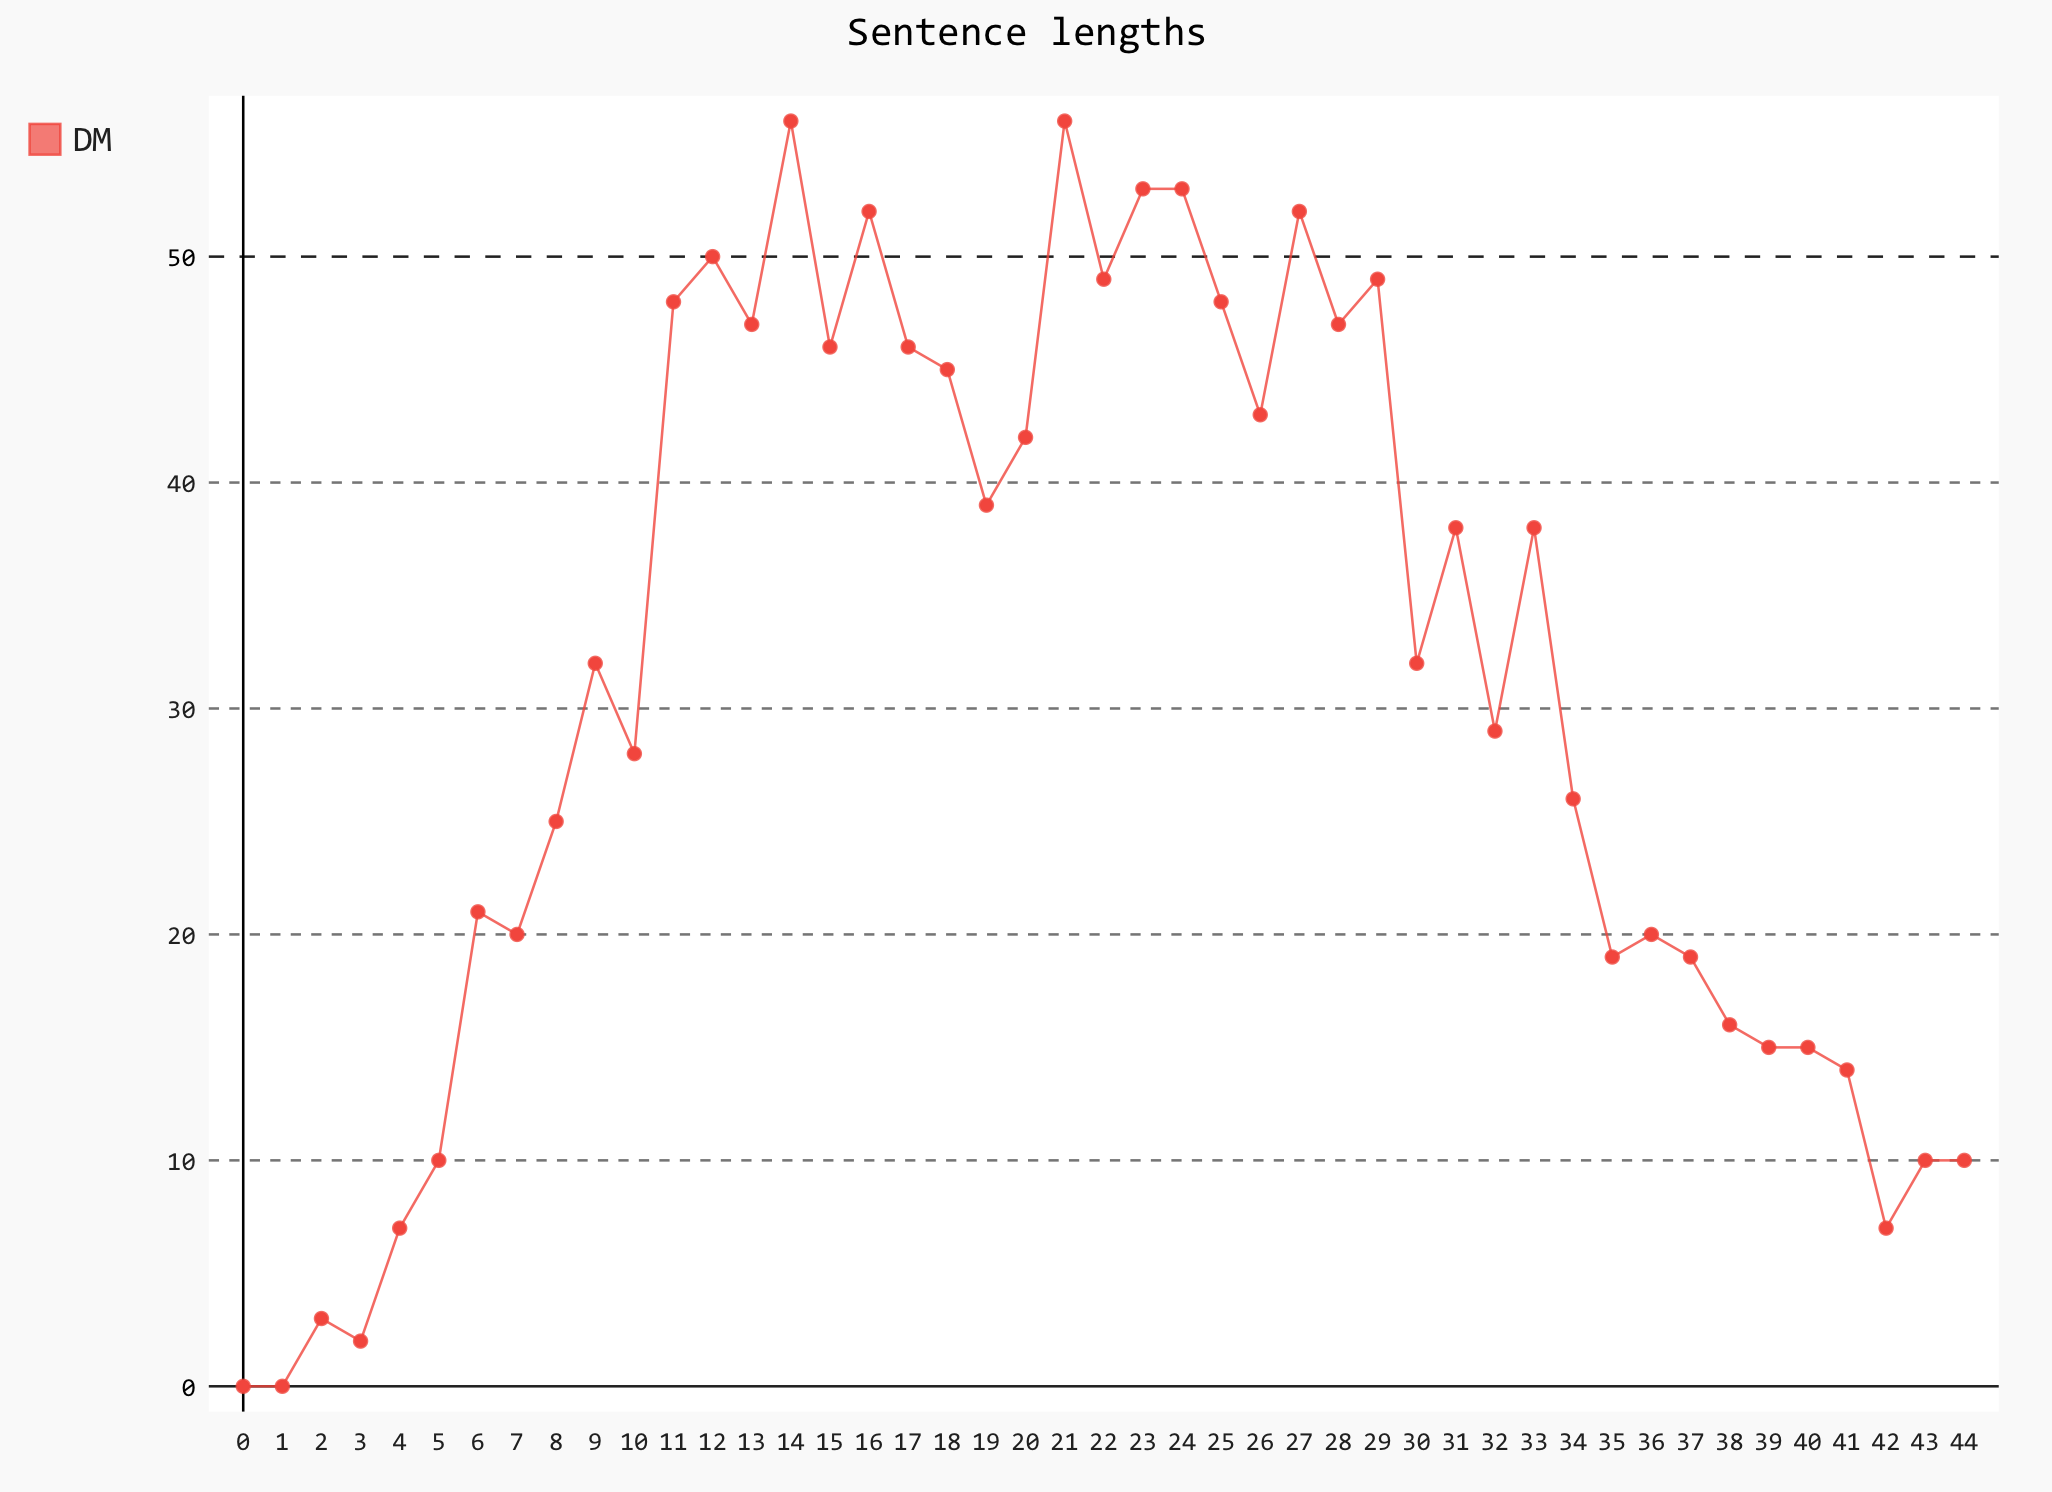
\includegraphics[width=\textwidth]{sentence_length}
% \label{fig:sentence_length}
% \end{figure}


\chapter{Semantic Frame Classification}
\label{chap:experiments}


We start this chapter by taking a closer look at the data sets that we use for training, developing and testing, through a set of experiments, a classifier for predicting semantic frames. The experiments and results of the classification will be presented in Chapter \ref{chap:results}. In this chapter we will focus on the feature selection and machine learning algorithms which serve as the foundation of our experiments. 

We use the DM and PSD target representations as basis for our experiments, and leave out PAS as it does not have semantic frames as part of its annotation scheme. This aligns with the analysis of the SemEval-2015 submissions from the previous chapter. We will also rely on the analysis of semantic frames from the previous chapter as basis for our feature selection.

The main part of this chapter will be dedicated to presenting the \textit{features} that we use as parameters for training our classifier. Features are individual properties that are either derived directly from the data sets, or by way of some transformation which can also include additional resources. The set of features we use for training our machine learning algorithms will determine their accuracy. We split our semantic frame classification into three different classifiers where the data used for training differentiates their outcome and usage:

\begin{enumerate}
    \item Classifying semantic frames based on \textit{lexical}, \textit{morphological} and \textit{syntactic} features.
    \item Classifying semantic frames based on \textit{lexical}, \textit{morphological} and \textit{semantic} features.
    \item Classifying semantic frames by combining the features of 1. and 2, i.e. using both syntactic and semantic features.
\end{enumerate}

The first set of experiments rely on information that does not rely on semantic dependency graphs. Our end result is a classifier where the predictions can be used as part of the feature space for training a semantic dependency parser. This could possibly increase the accuracy of state-of-the-art semantic dependency parsers. The second set of experiments leads to a classifier that relies on the results of a semantic dependency parser for its classification. We leave out syntactic information in this set of experiments in order to compare our results to the SemEval-2015 submissions that participated in the closed track. The last set of experiments would be a semantic frame classifier that relies on both a syntactic and semantic parser, and would be comparable to the parsing systems that participated in the SemEval-2015 open track.

In this chapter we will also present our experimental setup, i.e. how we prepare the data for training, development and testing. We will also provide overviews of the machine learning algorithms used as basis for our experiments. We have decided to run our experiments on \textit{Decision Trees}, \textit{Support Vector Machines}, \textit{Logistic Regression} and \textit{K-nearest neighbors}. This ensures a comparative basis for the choice of a machine learning algorithm as basis for our classifier.


\section{Experimental setup}
\label{setup}

\begin{table}
    \centering
    \smaller[0.2]
    \begin{tabular}{@{}llll@{}}
        \toprule
        \textbf{Type} & \textbf{\# Sentences} & \textbf{Frames} & \textbf{\# Frames} \\
        \midrule
        DM training & 28525 & 466 & 494122 \\
        DM development & 7131 & 378 & 123128 \\
        DM test id & 1410 & 290 & 24229 \\
        DM test ood & 1849 & 299 & 23486 \\
        \midrule
        PSD training & 28525 & 5074 & 72006 \\
        PSD development & 7131 & 2705 & 17387 \\
        PSD test id & 1410 & 1174 & 3673 \\
        PSD test ood & 1849 & 1265 & 3882 \\
        \bottomrule
    \end{tabular}
    \caption{The data sets used for training, development and testing. The test set consists of in domain (id) and out of domain (ood) data}
    \label{table:split}
\end{table}

\begin{table}
    \centering
    \smaller[0.2]
    \begin{tabular}{@{}llll@{}}
        \toprule
        \textbf{Type} & \textbf{\# Sentences} & \textbf{Frames} & \textbf{\# Frames} \\
        \midrule
        DM training & 28525 & 294 & 67493 \\
        DM development & 7131 & 231 & 16295 \\
        DM test id & 1410 & 162 & 3459 \\
        DM test ood & 1849 & 173 & 3750 \\
        \midrule
        PSD training & 28525 & 4951 & 69669 \\
        PSD development & 7131 & 2634 & 16761 \\
        PSD test id & 1410 & 1141 & 3584 \\
        PSD test ood & 1849  & 1209 & 3919 \\
        \bottomrule
    \end{tabular}
    \caption{The data sets used for training, development and testing, but excluding frames on the basis of the rules of the SemEval-2015 evaluation criteria.}
    \label{table:split:VandPred}
\end{table}


We have already explored the details of our data sets in Chapter \ref{chap:semantic}. In this section we focus on how we use the data to train, develop and test our machine learning models. As part of SemEval-2015, an official test data set was made available, and as such we do not need to set aside a test set for our final evaluation. In order to have a data set for tuning while we are experimenting with our feature selection, we need to set aside part of the training data for development purposes.

In Table \ref{table:split} we can observe some higher order statistics on the training, development and test data sets. We have split the original training set using an often used 80-20 split, where we extract 20\% of the training data for tuning and development purposes during our experimentation. This is to ensure that we do not run our experiments on the test data set, and thus avoid over-fitting our machine learning models by selecting features that increase the accuracy of our models directly on the test data.

Once we are ready to run a final set of tests, we will train our classifiers on the whole training set, including the held out development set used for tuning purposes, and observe the accuracy of our models on the official test set. This will then be presented as the final results of our classification task.

In Table \ref{table:split} we observe that the test data consists of in-domain and out-of-domain data. We will test our machine learning models on both these data sets in the final rounds of testing. Our hypothesis, based on the results of the SemEval-2015 submissions, and general intuition about machine learning, is that the accuracy of our classifier will be lower on the out-of-domain data sets.

Examining Table \ref{table:split} further, we see that the training data consists of 28525 sentences, the development data set of 7131 sentences, the in-domain test set of 1410 sentences and out-of-domain test set of 1849 sentences. For the DM target representation we observe a total of 494122 occurrences of frames in the training set, consisting of 466 unique frames. For the PSD training set, we observe 72006 occurrences of frames and a total number of 5074 unique frames. It is therefore important to note that due to the higher number of unique frames in the PSD data set, we can hypothesize that we will observe a relative drop in the accuracy of our classifier in comparison to the DM target representation.

In evaluating the performance of our models, we follow the SemEval-2015 scoring scheme, which was presented in Chapter \ref{chap:analysis}. In terms of only scoring frames that are not singletons, we do not use this information during training and classification. We train our model on all tokens that have a part of speech tag that starts with the character `V'. During classification we also predict semantic frames for all tokens that have a part of speech tag that starts with `V', but exclude tokens that are singletons as a post-processing step when we evaluate our models.

Now that we have some further insight into the data, and the experimental setup for our classification task, we present the feature selection that will function as basis for our experiments.

\section{Feature Selection}
\label{features}

\begin{figure}
    \centering
    \smaller[]
    \smaller[]
    \smaller[]
    % \tiny
    \begin{dependency}[]
        \begin{deptext}[column sep=0.5em, row sep=.1ex]
            Bramalea \& said \& it \& expects \& to \& complete \& the \& issue \& by \& the \& end \& of \& the \& month \& . \\
            
            g\_p\_n \& say \& it \& expect \& to \& complete \& the \& issue \& by \& the \& end \& of \& the \& month \& \_ \\
            
            NNP \& VBD \& PRP \& VBZ \& TO \& VB \& DT \& NN \& IN \& DT \& NN \& IN \& DT \& NN \& . \\
            
            named:x-c \& v\_to:e-i-h-i \& pron:x \& v:e-i-h \& \_ \& v:e-i-p \& q:i-h-h \& n:x \& p:e-u-i \& q:i-h-h \& n\_of:x-i \& \_ \& q:i-h-h \& n:x \& \_ \\
        \end{deptext}
        \deproot{2}{root}
        \depedge{2}{1}{ARG1}
        \depedge{6}{3}{ARG1}
        \depedge{4}{3}{ARG1}
        \depedge{2}{4}{ARG2}
        \depedge{9}{6}{ARG1}
        \depedge{4}{6}{ARG2}
        \depedge{6}{8}{ARG2}
        \depedge{7}{8}{BV}
        \depedge{9}{11}{ARG2}
        \depedge{10}{11}{BV}
        \depedge{11}{14}{ARG1}
        \depedge{13}{14}{BV}
    \end{dependency}
    \caption{DM target representation with tokens, lemma, part of speech tags, semantic frames and labeled semantic dependencies.}
    \label{DM:all}
\end{figure}

Feature selection is a process where we select the data that will be given to our machine learning algorithms as basis for its learning. For each token in the data, we extract a set of features that are used as input data for the machine learning algorithms as parameters for learning. During the training, each feature set has a corresponding semantic frame as its correct class. The machine learning will use this as basis for learning a mapping from a set of features to a correct semantic frame. Once a model has been trained, we can evaluate its performance by predicting classes for unseen tokens in the left out data used for development purposes. The score from this evaluation will be the basis for tuning, i.e. changing the set of features used for training.

There are no well defined methods by which we can empirically select the features that will result in the most accurate machine learning model. This is due to the fact that the feature space that is possible to construct is not finite, and we therefore have no way of testing all possible feature sets in order to find the set that will produce the most accurate classifier. We must therefore heuristically select our features by examining their impact on the accuracy of our classifiers.

When choosing features for our classifier we consider 3 factors:

\begin{enumerate}
    \item Improving accuracy: We aim for features that increase overall accuracy of our model.
    \item Reducing over-fitting: We create a development set so that we do not over-fit our features to the data.
    \item Reducing training and testing time: We employ a range of statistical measures for feature reduction so that we can increase the speed of training in order to run as many experiments as needed during our feature selection.
\end{enumerate}

We have chosen to base our feature selection on 4 sets of \textit{feature types}: lexical, morphological, syntactic and semantic. Examining Figure \ref{DM:all}, we have an example sentence taken from the training data which includes most of the information we will use as features. This example has been taken from the DM target representation. We start from the top of this figure. 

The first layer of information is the labeled semantic dependencies. We will use labeled dependencies as part of our feature space in the second and third classifier. For the second classifier we will use syntactic dependencies. For the syntactic dependencies we use the companion files distributed as part of SemEval-2015, where syntactic dependencies on the training and test data have been produced using the so-called Stanford Basic scheme derived from the Penn Treebank \cite{PennTreebank}. The parser of \citeA{Boh:Niv:12} have been used for the parsing.

In the next layer of information we have the \textit{token forms}, i.e. the words in their original form. The word forms are the units of information that are closest to the actual data (corpora), and the processing that has been performed in this layer is a tokenization step. For frame classification, we will use the token form as basis for our first set of experiments. However, as we will show in our experiments, using token form as our sole feature has its limitations, and with the size of our data and choice of machine learning algorithms, additional features are necessary in order to achieve state-of-the-art accuracy.

In the next layer of Figure \ref{DM:all}, we have the \textit{token lemma}. The \textit{lemma} of a word is its base representation. An example of this are the verbs `run', `runs', `ran' and `running', which are different word forms that share the same lemma `run'. Lemmatisation is a \textit{lossy} processing step whereby we lose some information by transforming words from one form to another. What we gain from processing tokens to find their base representation is a reduced vocabulary size, which in turn presents us with more coarse representations of a token and its context. The usage of lemma as features can thus increase classification accuracy for a set of tasks. However, some information is lost in this process, which for the case of semantic frame classification can lead to lower precision for tokens that are possibly mapped to a large set of semantic frames.

The layer below the token lemma, we have part of speech tags. These are grammatical categories, such as Nouns, Verbs, Adverbs, that have been assigned to the tokens of a sentence. Part of speech tags can help in disambiguation tasks when there is a possible link to a semantic frame for a token that has a set of possible frames where token form, or token lemma, fall short.

We will now examine how we will use these possible features in our experiments, and give definitions for these feature sets.

\subsection{Lexical and Morphological Features}

The lexical features that we will examine in our experiments are the \textit{token forms}, \textit{token lemmas} themselves, and \textit{prefixes} and \textit{suffixes} that we can derive form these. The information contained in word forms are the most fine grained information that resides in a sentence. The token forms are the information that acts as the basis for all the other features, which have been derive either directly, or indirectly, from these ground units. However, word forms suffer from the fact that in most corpora beyond a certain size, there will be a large set of infrequent word forms. It is therefore likely that using token forms will run into an issue of sparsity for infrequent ambiguous verbs that can be labeled with a range of semantic frames.

The lemma of a token will not fully resolve the sparsity connected to infrequent word forms. However, it will reduce the vocabulary of a corpora, and provide learning examples whereby a machine learning algorithm can connect an infrequent word form with its family of word forms, i.e. its lemma. However, for more frequent verbs, the disambiguation needed to distinguish between many classes of semantic frames, we might lose accuracy if we use lemma as a substitute for word form. A combination of form and lemma, which will be confirmed through our experimentation, is more likely to produce greater accuracy.

Prefixes and suffixes of word forms may introduce patterns in the data that may be useful for semantic frame classification. Our hypothesis is that, particularly suffixes, with such patterns as `ing', `ed', and `ang', may provide some additional information on the usage and context of a verb. However, these may also be too general too actually provide useful features for distinguishing between the correct semantic frame.

\subsection{Syntactic Features}

The syntactic features we will experiment with as part of our feature selection are the labeled dependencies in a syntactic dependency tree. Each sentence in the data set has a corresponding syntactic dependency tree. These trees are highly interesting in relation to our classification task. The semantic frame of a token is in many cases connected to the number of arguments a verb can take, and the type of dependency labels they have. Using the dependents of a token as a set of features may help distinguish between the various frames for ambiguous verbs where other features may be less relevant. Our experiments will include using the dependency labels in connection with the token form, token lemma, and the part of speech tag of the dependent.

We can also use the head of a token as its feature. Our hypothesis is that the heads of verbs do not add the necessary information that could possibly help in distinguishing their specific frame.

\subsection{Semantic}

For semantic features we are using the gold standard semantic graphs provided by the SemEval-2015 organizers in the DM and PSD target representations. In the same way as syntactic features, the semantic graphs can be useful in distinguishing frames by using the dependents in a semantic dependency graph. Examining Figure \ref{DM:all}, we can illustrate this by examining the verb `complete', which has two dependents: `it' and `issue', and where both have the labels `ARG1'. This indicates that this particular verb can have two dependents that are of \textit{type} `ARG1', which might distinguish it from other verbs used in the same context. When using dependents as features, we are faced with the possibility of having to sparse feature representations. Using the part of speech tags of dependents, instead of their form or lemma, can possibly help mitigate this, and lead to representations that are more informative for our classification.

Now that we have presented the possible feature space that we will use for our classification task, we will now examine the machine learning algorithms used as basis for our classification.

 
\section{Classification Algorithms}

We have chosen a set of four classifiers for predicting semantic frames in order to have a variety of approaches where we can empirically find a machine learning approach that yields satisfactory results. We start this chapter by providing a short description of the four algorithms that we have chosen for our classification task. These four machine learning algorithms are all implemented and openly available as part of the \textit{scikit-learn toolkit}.

Scikit-learn is a high-level machine learning toolkit written in the Python programming language. The authors of scikit-learn describe the toolkit as a set of state-of-the art machine learning algorithms that have been designed for usage on medium-scale supervised and unsupervised problems \cite{scikit-learn}. It well established machine learning toolkit that is both used in research and business.

It is worth noting that we ran the experiments on all four algorithms to a certain limit. Once we established the classifier that consistently performed with the highest accuracy on our chosen set of initial features, we limited further explorations to the most accurate algorithm. Since running the experiments on each classifier is time consuming, this decision was necessary once we started performing more in-depth feature selections so that we could proceed in a timely fashion. Our aim is to examine the possibilities of increasing the accuracy of frame detection to rival that of the current state-of-the-art.

\subsection{Decision Trees}

\textit{Decision Tree Classifiers} learn rules by creating a tree structure with simple rules that are easy to analyze and understand. This can be contrasted to more complex machine learning algorithms such as \textit{neural networks}. In the latter cases the learning and predictions made by the algorithm acts like a `black-box' in terms of comprehensibility.

The decision tree algorithm learns based on a set of labeled instances by inductively setting up a set of rules which form a tree structure. The tree structure can be visualized by thinking of each node in the tree as a question. Classification is done by starting at the root node, and based on the rules that have been learned, classify new data by traversing the tree and reaching a node that is designated by a specific class. For each node, a check is made on the unseen data that is to be labeled as the traversing step. As Kotsiantis note, the process by which a decision tree classifier makes predictions is similar to a greedy search \cite{Kotsiantis:13}.

The decision tree classifier that is part of the scikit-learn toolkit has a small set of options for creating different types of decision trees. The options include setting the split criteria, where the options are \textit{gini} and \textit{entropy}. As Kotsiantis note, gini and entropy are two different measure used as the splitting measure that the learning algorithm uses in order to create the decision trees \cite{Kotsiantis:13}.

Our experiments showed that decision trees can be a fast and accurate machine learning algorithm for frame classification. However, it did not score high enough to be considered for further exploration beyond the morphological features described in Section \ref{features}. We also observed that the high dimensionality of features used in our classifier was not suited for a decision tree classifier.

\subsection{Support Vector Machines}

\textit{Support vector machines} are well suited for multi-class classification tasks, particularly when dealing with high dimensional feature sets as in our case. As Hsu and Lin note, at the time when support vector machines where created it was initially made for binary classification. However, a number of methods have been constructed whereby a support vector machine can be extended to handle multiple classes \cite{Hsu:02}.

The scikit-learn toolkit has 3 implementations of support vector machines. After a few experiments, we ended up using the `LinearSVC' class, which is a wrapper around the `LIBLINEAR' library developed by  \citeA{liblinear}. Without parameter tuning, this implementation proved the most accurate on our initial set of experiments. We not include the experiments run on the other implementations that are part of the scikit-learn tookit.

The `LIBLINEAR' library is an open source library for large-scale linear classification. It is well suited for large data and feature sets, and it is particularly recommended for text classification by its developers. In certain cases it is also known to be faster than many support vector implementations, including the often used `LIBSVM' library \cite{liblinear}. The other scikit-learn support vector machine algorithms are based on `LIBSVM', which proved to be relatively slower once our feature sets grew to include syntactic and semantic features. We found that by using the `LinearSVC' class in the scikit-learn toolkit we reduce training time, which made it possible to run more experiments in comparison with the other implementations. 

Our experiments showed that support vector machines had the highest overall scores among the four machine learning algorithms on the first set of morphological features. It is a versatile algorithm that performed well without any parameter tuning. We therefore opted for this algorithm once we reached a threshold of experimentation on the basis of its comparatively higher accuracy. It is not definite that the other machine learning algorithms could not produce comparable, or even higher accuracy. However, this would have demanded a greater effort in examining the possible range of parameter tuning for all four algorithms, which unfortunately was deemed outside the scope of our thesis.

\subsection{Logistic Regression}

Logistic regression is a machine learning model based on regression analysis. The implementation used in scikit-learn, like the support vector machine implementation described above, is based on the `LIBLINEAR' library. The implementation is of a multivariate logistic regression model with the loss function being $log(1+e^{y_iw^Txi})$, which has been derived from a probabilistic model \cite{liblinear}. 

We achieved relatively high accuracy using the logistic regression model at a training time that allowed for experimentation with different feature sets. However, as we saw that the support vector implementation scored relatively higher for all lexical and morphological features, we did not further test this algorithm once we started experimenting with syntactic and semantic features. It is our hypothesis that with devoted analysis to the effects of parameter tuning, logistic regression could potentially be an interesting rival to support vector machines for our case. This is based on the fact that logistic regression and support vector machine implementations showed relatively similar accuracy levels on most of the experiments we ran on both algorithms.

\subsection{K-nearest neighbors}

Nearest neighbors classification is a type of machine learning method where training data is stored directly in a model, and a computation is performed by way of a simple majority vote of the nearest neighbors of each point in the model. It is a non-parametric method used for both classification and regression, where in the classification the output of our model is a class, and in regression the output is the average of the values of its \textit{k} neighbors \cite{Altman:92}. The k-nearest neighbors algorithm can also be used as an unsupervised learning algorithm, and is often used as basis for tasks that involve some form of clustering.

We did not achieve comparably high accuracy using the k-nearest neighbors classifier implemented in the scikit-learn toolkit. We therefore opted to leave out this algorithm as well once we started our experiments with syntactic and semantic features. In fact, for high feature dimensions, the accuracy of this algorithm performed well below the other three algorithms we examined.

\section{Conclusions}

In this chapter we have reviewed our experimental setup. We have presented the training, development, and test data, and given an overview of the distribution of semantic frames across these sets. We have also presented the feature types that we will use as basis for our experiments, and the machine learning algorithms that we will examine as basis for creating our classifiers. In the next chapter we will present the results of our feature selection and experiments with different machine learning techniques. We show that with in-depth feature selection, it is possible to rival the accuracy of state-of-the-art semantic frame classification, and that our results can be used as basis for enhancing the best submissions in the closed track of SemEval-2015.
\chapter{Experiments}
\label{chap:results}

% random baseline
% most frequent class vs most frequent per lemma
% the latter is a strong baseline
% PSD, multiclass classification is good for PSD, it is noteworthy. 
% For PSD Praha uses a classificator for each lemma
% Sanity test for lemma test
% why is lemma and form higher for PSD. Tense may play a greater role in PSD. 
% surface instead of lexical
% n-gram to window
% form-window
% could have done things in a more greedy fashion, but we used a method where we build upon previous results
% syntactic - label + pos, just labels
% semantic - label + pos, just labels
% SVM undemanding in terms of parameter tuning

In this chapter we will examine and present experimental results for the task of frame classification. We will use the data sets presented in Chapter \ref{chap:analysis}, and \ref{chap:experiments} for training, development and testing. We will examine how each set of features impacts the precision, recall and F-score of our models. The mathematical definitions of these measures can be found in Chapter \ref{chap:analysis}. The end result of our experiments will be two different semantic frame classifiers based on the feature sets used for training. Both classifiers share the same lexical and morphological features, but diverge in using syntactic and semantic dependencies as additional features on top of these. Once we have finished our experiments on the development data set, we present our final results on the test data. Our results show that with rigorous experimentation with different combination of features, we were able to obtain state-of-the-art results for semantic frame classification. We compare our results with previous results in frame classification. We also show that by extending two of the participating systems of SemEval-2015, namely Lisbon and Peking, our results can be used to improve these system's semantic frame classification accuracy.


\section{Baseline}

Before we start our experiments, we need to define a baseline in order to have a common denominator that we can evaluate our results against. There are no agreed upon standards for defining a baseline for classification tasks such as semantic frame classification. Statistical counting measures have been the standard in other tasks, such as \textit{part of speech tagging}. We will draw inspiration from methods used in part of speech tagging for setting up a baseline for our task.

\begin{table}
    \centering
    \smaller[0.2]
    \begin{tabular}{@{}lllll@{}}
        \toprule
        \textbf{Representation} & \textbf{Precision} & \textbf{Recall} & \textbf{F-score} \\
        \midrule
        DM & 72.09 & 73.70 & 71.76\\ 
        PSD & 58.63 & 66.55 & 61.47\\
        \bottomrule
    \end{tabular}
    \caption{Baseline score with a most frequent frame per lemma approach.}
    \label{table:baseline}
\end{table}

An often used baseline in part of speech tagging is a \textit{most frequent class} approach: given an ambiguous word, assign to it the most frequent part of speech tag \cite{Jur:Mar:09}. In part of speech tagging most words are unambiguous (80-86\%), and we are therefore left with approximately 14-15\% of words where using the most frequent tag for for said word will results in possible errors. Running a most frequent class baseline classifier for part of speech tagging on the WSJ corpus results in an accuracy of 92.34\% \cite{Jur:Mar:09}. State-of-the art part of speech taggers have been able to achieve accuracy scores above 97\%, which is a significant increase from the baseline.

Examining Tables \ref{table:dm_frames_freq} and \ref{table:psd_frames_freq} in Chapter \ref{chap:analysis}, we observe that the ten most frequent frames in both data sets account for 18.64\% and 9.35\% of all frames respectively. Given the number of frames and their distribution, we will use the same approach as part of speech tagging and use a \textit{most frequent class per lemma} approach for our baseline. For each lemma in the development set, we assign to it the most frequent frame encountered for that lemma in the training set. For lemmas that have not been encountered in the training, we assign the overall \textit{most frequent frame} in the training data. This approach results in a \textit{strong} baseline. A \textit{weak} baseline would be a baseline where we assigned the most frequent frame to all tokens. Another option, which would also be a weak baseline, is a \textit{random} baseline where we randomly assign frames to each token.

In Table \ref{table:baseline}, we have listed the baselines using the most frequent frame per lemma approach. It is worth reminding that we evaluate the baseline, as with all experiments in this chapter, by only including tokens that have a part of speech tag that starts with the character `V' and is not a singleton. However, we can only access the part of speech tag information during training and prediction, and it is only after classification that we use information that a token is a singleton or not, based on the gold standard data, for scoring. A detailed description of the scoring scheme is described in Chapter \ref{chap:analysis}.

We observe that the baseline for DM is significantly higher than PSD. We explain this discrepancy by noting that the PSD target representation consists of a much larger set of frames. If we examine frequent lemmas, such as `be', `make', 'have', `take', `say', we observe that for these verbs, the number of frames assigned in the PSD target representations is higher, and the distribution of the frames assigned are more uniform. A most frequent frame per lemma approach will therefore be less effective for the PSD target representation.

Now that we have established a baseline we start with our first set of experiments using \textit{lexical} and \textit{morphological} features for training. We then go on to examining \textit{syntactic} dependencies as features, resulting in our first semantic frame classifier. After syntactic features we will introduce the results of using \textit{semantic} dependencies as features, resulting in our second classifier.



\section{Experiments}

We start things off by examining a set of features in order to establish some basic information on the results we can obtain on the four machine learning algorithms we will examine. With this information at hand we choose one of these four algorithms to continue our experiments with. We start by examining lexical features and observe the scores we can obtain by solely using these so-called surface features. 

% We then continue to examine morphological features. Here we will examine part of speech tags, suffixes and prefixes. We then go on to examining syntactic and semantic dependencies. Once we have reached a saturation point in our feature selection, we run our final models on the test set and report our results. As a final step we compare our results to the SemEval-2015 submissions.

% We also use this as basis for choosing which of the four machine learning algorithms we will continue using as basis for further experiments with multiple features.


\subsection{Lexical Features}
\label{results_lex}

\begin{table}
    \centering
    \smaller[0.2]
    \begin{tabular}{@{}clllll@{}}
        \toprule
        & \textbf{Classifier} & \textbf{Precision} & \textbf{Recall} & \textbf{F-score} \\
        \midrule
        \multirow{5}{*}{\rotatebox[origin=c]{90}{\bfseries\textsc{DM}}}
        & Baseline & 72.09 & 73.70 & \textbf{71.76}\\ 
        & Support Vector Machine & 70.85  &  70.98  &  69.58  \\
        & Decision Tree & 71.05  &  70.89  &  69.60 \\
        & Logistic Regression & 67.04  &  68.00  &  65.34 \\
        & K-Nearest Neighbor & 69.32  &  63.44  &  65.00 \\
        \midrule
        \multirow{5}{*}{\rotatebox[origin=c]{90}{\bfseries\textsc{PSD}}}
        & Baseline & 58.63 & 66.55 & 61.47\\
        & Support Vector Machine & 66.91  &  66.88  &  \textbf{64.83} \\
        & Decision Tree & 66.79  &  66.76  &  64.72 \\
        & Logistic Regression &  62.11 &   60.57 &   59.33 \\
        & K-Nearest Neighbor & 64.34  &  64.10  &  62.74 \\
        \bottomrule
    \end{tabular}
    \caption{Results for \textit{form} as the sole feature.}
    \label{table:form}
\end{table}

\begin{table}
    \centering
    \smaller[0.2]
    \begin{tabular}{@{}clllll@{}}
        \toprule
        & \textbf{Classifier} & \textbf{Precision} & \textbf{Recall} & \textbf{F-score} \\
        \midrule
        \multirow{5}{*}{\rotatebox[origin=c]{90}{\bfseries\textsc{DM}}}
        & Baseline & 72.09 & 73.70 & 71.76\\ 
        & Support Vector Machine & 71.79    & 74.20    & \textbf{71.81}  \\
        & Decision Tree & 71.67  & 74.12    & 71.74 \\
        & Logistic Regression & 69.97    & 72.98    & 70.00 \\
        & K-Nearest Neighbor & 69.61    & 68.18    & 67.60 \\
        \midrule
        \multirow{5}{*}{\rotatebox[origin=c]{90}{\bfseries\textsc{PSD}}}
        & Baseline & 58.63 & 66.55 & \textbf{61.47}\\
        & Support Vector Machine & 58.55    & 66.47    & 61.39 \\
        & Decision Tree & 58.60 &  66.52    & 61.44 \\
        & Logistic Regression  & 55.43    & 63.22    & 58.23 \\
        & K-Nearest Neighbor & 55.69    & 63.30    & 58.40 \\
        \bottomrule
    \end{tabular}
    \caption{Results for \textit{lemma} as the sole feature}
    \label{table:lemma}
\end{table}

\begin{table}
    \centering
    \smaller[0.2]
    \begin{tabular}{@{}clllll@{}}
        \toprule
        & \textbf{Classifier} & \textbf{Precision} & \textbf{Recall} & \textbf{F-score} \\
        \midrule
        \multirow{5}{*}{\rotatebox[origin=c]{90}{\bfseries\textsc{DM}}}
        & Baseline & 72.09 & 73.70 & 71.76\\ 
        & Support Vector Machine & 75.67 & 74.01 & \textbf{72.68} \\
        & Decision Tree & 75.80 & 73.78 & 72.48 \\
        & Logistic Regression & 71.35 & 72.93 & 71.00 \\
        & K-Nearest Neighbor & 74.96 & 72.55 & 72.23 \\
        \midrule
        \multirow{5}{*}{\rotatebox[origin=c]{90}{\bfseries\textsc{PSD}}}
        & Baseline & 58.63 & 66.55 & 61.47\\
        & Support Vector Machine & 70.34 & 70.86 & \textbf{68.62} \\
        & Decision Tree & 69.86 & 70.10 & 68.02 \\
        & Logistic Regression  & 67.66 & 68.55 & 66.20 \\
        & K-Nearest Neighbor & 66.97 & 68.70 & 66.36 \\
        \bottomrule
    \end{tabular}
    \caption{Results for \textit{form} and \textit{lemma} as features}
    \label{table:form_lemma}
\end{table}

\begin{table}
    \centering
    \smaller[0.2]
    \begin{tabular}{@{}clllll@{}}
        \toprule
        & \textbf{Classifier} & \textbf{Precision} & \textbf{Recall} & \textbf{F-score} \\
        \midrule
        \multirow{5}{*}{\rotatebox[origin=c]{90}{\bfseries\textsc{DM}}}
        & Baseline & 72.09 & 73.70 & 71.76\\ 
        & Support Vector Machine & 85.20 & 84.44 & \textbf{84.10} \\
        & Decision Tree & 78.49 & 76.90 & 76.73 \\
        & Logistic Regression & 82.22 & 80.69 & 79.54 \\
        & K-Nearest Neighbor & 64.33 & 55.83 & 57.45 \\
        \midrule
        \multirow{5}{*}{\rotatebox[origin=c]{90}{\bfseries\textsc{PSD}}}
        & Baseline & 58.63 & 66.55 & 61.47\\
        & Support Vector Machine & 80.09 & 80.38 & \textbf{79.09} \\
        & Decision Tree & 77.51 & 74.19 & 74.53 \\
        & Logistic Regression & 71.31 & 71.90 & 69.85 \\
        & K-Nearest Neighbor & 44.14 & 37.05 & 37.24 \\
        \bottomrule
    \end{tabular}
    \caption{Results for \textit{form} and \textit{lemma} on the main verb token, and a context window of $n=3$ where we use \textit{token form} as the window.}
    \label{table:form_lemma_context=3}
\end{table}

\paragraph{Token Form} The first feature we will examine is the \textit{form} of verb tokens. For each token that is a verb, we use its form as the sole feature for classifying the frame of that token. In Table \ref{table:form} we have listed the results using this feature on the four machine learning algorithms we are experimenting with. It is interesting to note that for the PSD target representation we achieve higher F-score than the baseline on all machine learning algorithms with the exception of Logistic Regression. However, with the exception of Support Vector Machines, we also observe that we achieve lower recall than the baseline. This might be due to the relative uniform distribution of frames on ambiguous verbs in PSD, and as such a most frequent frame per lemma baseline will have a higher recall than precision. In comparison, we observe that the difference between precision and recall is much higher for PSD than DM.

The scores for the DM target representation are approximately 3 to 7 percentage points lower than the baseline. This is due to the fact that we are using the tokens form, as opposed to the lemma, which is what we have used in our baseline.

\paragraph{Token Lemma} In our next run we will examine how using \textit{lemma} as the sole feature, in the same way as in our baseline, impacts the learning. The results are presented in Table \ref{table:lemma}. We observe that the results are overall higher than using form as our sole feature for the DM target representation, but lower for PSD. Our hypothesis is that this is, as with our baseline score, an artifact of the number and distribution of frames across the target representations. 

% We also attempted, for experimental purposes, to test our classifier with \textit{part of speech tags} as the sole feature. Our hypothesis was that we would achieve low results due to the fact that the disambiguation needed for semantic frame detection does not correlate strongly with part of speech tags. We will not report the numbers in a table, as they are not interesting as a comparison to the other results, but we note that the F-scores where all below 30\% for the 4 machine learning models. However, this does not mean that part of speech tags are not interesting as features for our models. In conjunction with lexical and other morphological features, we will show that part of speech tags in fact contribute to higher scores when we get to our section on morphological features.

\paragraph{Combination of Form and Lemma} Let us now turn to combining lexical features. We start by examining whether the combination of form and lemma results in a higher score in comparison to using form or lemma in isolation. In Table \ref{table:form_lemma} we see that we achieve a slight increase for the DM target representation when compared to the results using just lemma, but a significant increase in PSD. The combination of the form and lemma of a token will has the information needed to achieve higher scores than the baseline.

\paragraph{Context Window} For our next experiment we examine how the context window of a token, referred to as \textit{token n-grams}, might impact the accuracy of our machine learning models. We will present experiments using a context window of 3 tokens surrounding the main token: `form-3', `form-2', `form-1', `form', `form+1', `form+2', `form+3'. The words are added as individual features using a bag-of-words approach, so order does not have an impact. This is done so that we avoid too sparse vectors that would have been the results of using concatenated tokens as features. Had we concatenated the words so that the word order was kept intact, we would end up with very infrequent strings, i.e. sparse features. In Table \ref{table:form_lemma_context=3} we see the results of our run with a context window of $n=3$, meaning that we have used 3 tokens to the left, and 3 tokens to the right, of our main verb token.

For the single features that we experimented with previously, the differences in results between the machine learning algorithms were less obvious. However, once we use a combination of features we observe that there is a higher degree of divergence. The Support Vector Machine algorithm achieves the highest score for both DM and PSD when using a context window by a significant margin. If we look at Table \ref{table:form_lemma_context=3}, we see that the F-score for DM for Support Vector Machine is 84.10\%, an increase from an F-score of 72.68\% in the previous experiments where we used form and lemma of the main token. For PSD we see an increase from an F-score of 68.62\% to 79.09\%. It is interesting to note that for the K-Nearest Neighbor Classifier we observed a decrease in score in comparison with previous results. 

The lower scores for the other algorithms was observed on all the experiments that are presented in this chapter. We therefore leave out these results from our presentation in order to keep the tables and presentation more compact and readable. However, it is worth noting that parameter tuning has not been performed in this study. It is therefore not possible to empirically argue that our choice in using Support Vector Machines leads to the most accurate classifier. For that we would need to perform an in-depth comparative study where we performed a range of tuning exercises for each algorithm. However, we deemed this outside the scope of our thesis.

\paragraph{Increased Context Window} Let us now increase the context window with a larger $n$, and use both \textit{form} and \textit{lemma} as basis for the surrounding $n$ elements. We will examine their performance both individually and in conjunction. Our context window for our experiments will be ${\{n|n>2 \wedge n<8\}}$. Tables \ref{table:form_context}, \ref{table:lemma_context}, and \ref{table:form_lemma_context}, show the results for ${\{n|n>2 \wedge n<6\}}$, for form, lemma and both respectively. 

Table \ref{table:form_context} shows the results for a context window consisting of form. We see an increase in F-score from $n=3$ to $n=4$, for both the DM and PSD target representations. We then observe a decrease once we reach $n=5$ for the context window. This decrease continued as $n$ increase. We omit these scores so that our tables are more readable.

In Table \ref{table:lemma_context} we observe a similar trend. The best results are for $n=3$, and we observe a higher score in comparison to Table \ref{table:form_context} where we used form in our context window. When we combine form and lemma, as seen in Table \ref{table:form_lemma_context}, we do not get higher scores than using just lemma.

For the context window, we observe that the best feature set for our task is using lemma with a context window of $n=3$. For our experiments going forward this will be the base configuration. The results for this set of features are an F-score of 86.58\% for DM and 83.20\% for PSD. These are the highest scores achieved thus far. We now turn to syntactic dependencies and examine their impact on the accuracy of our system.

\begin{table}
    \centering
    \smaller[0.2]
    \begin{tabular}{@{}lllll@{}}
        \toprule
        \textbf{Representation} & \textbf{N-gram} & \textbf{Precision} & \textbf{Recall} & \textbf{F-score} \\
        \midrule
        DM & $n=3$ & 85.20 & 84.44 & 84.10 \\
        DM & $n=4$  & 87.17 & 86.52 & \textbf{86.32} \\
        DM & $n=5$  & 86.88 & 86.20 & 85.99 \\
        \midrule
        PSD & $n=3$ & 80.09 & 80.38 & 79.09 \\
        PSD & $n=4$ & 83.20 & 83.66 & \textbf{82.41} \\
        PSD & $n=5$ & 82.54 & 83.09 & 81.73 \\
        \bottomrule
    \end{tabular}
    \caption{Results for experiments with context windows of ${\{n|n>2 \wedge n<6\}}$ using only \textit{form} as the context window.}
    \label{table:form_context}
\end{table}

\begin{table}
    \centering
    \smaller[0.2]
    \begin{tabular}{@{}lllll@{}}
        \toprule
        \textbf{Representation} & \textbf{N-gram} & \textbf{Precision} & \textbf{Recall} & \textbf{F-score} \\
        \midrule
        DM & $n=3$ & 87.34 & 86.67 & \textbf{86.58} \\
        DM & $n=4$  & 87.07 & 86.46 & 86.32 \\
        DM & $n=5$  & 86.7 & 86.12 & 85.97 \\
        \midrule
        PSD & $n=3$ & 83.88 & 84.39 & \textbf{83.20} \\
        PSD & $n=4$ & 83.55 & 84.07 & 82.79 \\
        PSD & $n=5$ & 83.01 & 83.61 & 82.25 \\
    
        \bottomrule
    \end{tabular}
    \caption{Results for experiments with context windows of ${\{n|n>2 \wedge n<6\}}$ using only \textit{lemma} as the context window.}
    \label{table:lemma_context}
\end{table}

\begin{table}
    \centering
    \smaller[0.2]
    \begin{tabular}{@{}lllll@{}}
        \toprule
        \textbf{Representation} & \textbf{N-gram} & \textbf{Precision} & \textbf{Recall} & \textbf{F-score} \\
        \midrule
        DM & $n=3$ &  87.08 & 86.43 & \textbf{86.29} \\
        DM & $n=4$  & 86.51 & 86.05 & 85.79 \\
        DM & $n=5$  & 86.34 & 85.86 & 85.59 \\
        \midrule
        PSD & $n=3$ & 83.39 & 83.98 & \textbf{82.71} \\
        PSD & $n=4$ & 82.80 & 83.48 & 82.10 \\
        PSD & $n=5$ & 82.37 & 83.26 & 81.81 \\
        \bottomrule
    \end{tabular}
    \caption{Results for experiments with context windows of ${\{n|n>2 \wedge n<6\}}$ using \textit{lemma} and \textit{form} as the context window.}
    \label{table:form_lemma_context}
\end{table}




\subsection{Morphological Features}
\label{results_morph}

The morphological features included in our experiments are part of speech tags, suffixes and prefixes. We will examine their impact on the accuracy of our classifier by examining each individually, and then adding the features that have the highest impact in a similar fashion as the lexical experiments. 

% \paragraph{Part of Speech Tags} For experimental purposes, we test our classifier with \textit{part of speech tags} as the sole feature. Our hypothesis is that we will achieve low results due to the fact that the disambiguation needed for semantic frame detection does not correlate strongly with part of speech tags as the sole feature. We do not report the numbers in a table, as they are not interesting as a comparison to the other results, but we note that F-scores are all below 30\% for the 4 machine learning models. However, this does not mean that part of speech tags are not interesting as features for our models. In conjunction with lexical and other morphological features, we will show that part of speech tags in fact contribute to higher scores when we get to our section on morphological features.

\paragraph{Part of Speech Tags with Form and Lemma} We will now examine the effects of adding part of speech tags to the form and lemma tokens. We will concatenate the tags at the end of each token: <form\_pos> and <lemma\_pos>. The results of our experiments are presented in Table \ref{table:pos}. In the first experiment, we concatenate the part of speech tag to the form token, leaving lemma as a feature on its own. We then do the opposite, concatenating the part of speech tag to the lemma, but leaving form as its own feature. We then concatenate the part of speech tag to both form and lemma. As a final run we combine all of the above: form and lemma as their own features, form and lemma concatenated with part of speech tag, and part of speech tag as its own separate feature. 

From Table \ref{table:pos}, we observe that the various strategies of using part of speech tags yield similar results. We see that the two highest scores, for both DM and PSD, are when we either concatenate part of speech tags to form, and leave lemma as a separate feature, or when we leave both form and lemma as a separate features, and the part of speech tag as its own separate feature. However, overall, the increase in precision, recall and F-score are relatively low in both cases, where for DM we see an increase from the previous best score of 86.58\% to 86.92\%, and 82.71\% to 83.27\% for PSD.

The increase is likely caused by the disambiguation possible for verbs that are assigned a range of different part of speech tags, such as the verb `make', which have been assigned this set of tags: `VB', `VBZ', `VBG', `VBD', `VBN', `VBP'. The uniform distribution of frames for each token in PSD might account for the greater increase in f-fscore when using part of speech tags.

\paragraph{Part of Speech Tags Added to the Context Window} We will now examine how part of speech tags may affect the accuracy of our model by adding them to the context window. We will run 2 set of experiments: (1) adding part of speech tags to the context window for the token lemma. This is done by concatenating them to the lemma as in our previous experiments. We also run experiments by adding the part of speech tags as separate features. The results are reported in Table \ref{table:pos_context}. Similar to the results in Table \ref{table:pos}, we observe that using part of speech tags as separate features for the context window results in the highest increase in F-score. 

The score once we have added part of speech tags are 88.08\% for DM and 84.02\% for PSD. With part of speech tags we have achieved an increase in our scores with 1.5 for DM and 0.82 percentage points for PSD. We therefore include these from this point on.

\paragraph{Prefixes and Suffixes} We will now consider adding prefixes and suffixes as features. For prefixes and suffixes we add character n-grams where ${\{n|n>2 \wedge n<5\}}$. This ensures that we capture various types of prefixes and suffixes that may be constrained by character length, such as the suffixes `ing' and `ed'. It is difficult estimating the effect of adding such morphological features, as the increase in our score is minimal. In Table \ref{table:affix_suffix} we observe that using only prefixes has an impact where we see an increase in F-score. The other experiments had a negative impact on the scores.

At this point it is worth mentioning that we may have reached a saturation point in the effects that new layers of features may have. In fact, if we had added part of speech tags, or even prefixes and suffixes, at an earlier stage, we might have concluded that some lexical features did not have an effect on the accuracy. Another set of experiments would be to test each set of features on their own, and then examine their cumulative effect after observing their effects on their own. We decided to run our experiments in sequence by adding features as we ran our experiments as we observed an effect of adding features for the most part.



\begin{table}
    \centering
    \smaller[0.2]
    \begin{tabular}{@{}llllll@{}}
        \toprule
        \multicolumn{3}{c}{DM}
        & \multicolumn{3}{c}{PSD} \\
        \textbf{Precision} & \textbf{Recall} & \textbf{F-score} & \textbf{Precision} & \textbf{Recall} & \textbf{F-score} \\
        \midrule
        87.46 & 86.81 & 86.71 & 84.04 & 84.40 & \textbf{83.30} \\
        86.46 & 85.85 & 85.69 & 81.66 & 81.91 & 80.76 \\
        86.23 & 85.63 & 85.45 & 80.79 & 80.91 & 79.81 \\
        87.67 & 87.00 & \textbf{86.92} & 84.00 & 84.43 & 83.27 \\
        86.18 & 85.54 & 85.37 & 80.71 & 80.87 & 79.76 \\
        \bottomrule
    \end{tabular}
    \caption{Results for adding part of speech tags: concatenated to form (first), concatenated to lemma (second), concatenated to both form and lemma (third), as a feature on its own (fourth), and concatenated to both form and lemma, form and lemma as features on their own, and part of speech tag as a feature on its own (fifth).}
    \label{table:pos}
\end{table}


\begin{table}
    \centering
    \smaller[0.2]
    \begin{tabular}{@{}llllll@{}}
        \toprule
        \multicolumn{3}{c}{DM}
        & \multicolumn{3}{c}{PSD} \\
        \textbf{Precision} & \textbf{Recall} & \textbf{F-score} & \textbf{Precision} & \textbf{Recall} & \textbf{F-score} \\
        \midrule
        87.67 & 87.00 & 86.92 & 84.00 & 84.43 & 83.27 \\
        88.52 & 88.27 & \textbf{88.08} & 84.24 & 85.51 & \textbf{84.02} \\
        88.51 & 88.26 & 88.07 & 84.25 & 85.52 & \textbf{84.02} \\
        \bottomrule
    \end{tabular}
    \caption{Results for adding part of speech tags to the context window, concatenating to lemma (top), as their own separate features (middle), and a combination of both, where we have lemma as their own features, part of speech as their own features, and part of speech tags concatenated to the lemma (bottom).}
    \label{table:pos_context}
\end{table}

\begin{table}
    \centering
    \smaller[0.2]
    \begin{tabular}{@{}llllll@{}}
        \toprule
        \multicolumn{3}{c}{DM}
        & \multicolumn{3}{c}{PSD} \\
        \textbf{Precision} & \textbf{Recall} & \textbf{F-score} & \textbf{Precision} & \textbf{Recall} & \textbf{F-score} \\
        \midrule
        88.69 & 88.29 & \textbf{88.20} & 84.13 & 85.53 & \textbf{83.99} \\
        88.37 & 88.03 & 87.89 & 83.69 & 85.05 & 83.50 \\
        88.56 & 88.15 & 88.06 & 84.06 & 85.42 & 83.89 \\
        \bottomrule
    \end{tabular}
    \caption{Results for adding prefix to the main form (first), suffixes to main form (second), both prefixes and suffixes to main form (third).}
    \label{table:affix_suffix}
\end{table}






\subsection{Syntactic Features}
\label{results_syn}

% previous
% 88.08\% for DM and 84.02\% for PSD


Syntactic dependencies are a very interesting set of features for frame detection. Ambiguous verbs such as `be', `make', 'have', `take', `say', have a variable set of syntactic dependencies that may have a relationship with their assigned semantic frames.

Let us examine two sentences from our training set: (1) `It has no bearing on our work force today' and (2) `They have to do it'. In sentence (1) the frame for the verb `has' is `v:e-i-i', indicating that it is a verb that can take two objects, whereas in sentence (2) the verb has been assigned the frame `v\_qmodal:e-h', which is an indication that it is a modal auxiliary verb to the verb `do'. The frames are from the DM target representation. In such examples the syntactic dependencies, i.e. their edges and labels, can function as parameters for distinguishing between these two type of frames. If we examine the type of errors that our previous experiments produce, it is these type of ambiguous verbs that account for a high percentage of errors.

For syntactic dependencies we will add the dependencies of the target token. We will add dependents by concatenating lemma and label: <lemma\_label>. The main verb of a dependency usually has several dependents, so we concatenate them all to a string as its own feature, sorting them by the dependency label in lexical order. 

As an example, for the token `join' we would have the string: <will\_aux: board\_obj: Vinken\_nsubj>, as a feature. However, concatenating dependency labels for the lemma will produce sparse features. We will also examine the effect of adding the head of our main tokens in the same way as our dependents, with the exception that we always have at most one syntactic head, and we therefore add the head's lemma and label concatenated as its own feature. 

We also do a combination of adding head and the dependents. The results of these experiments are seen in Table \ref{table:dependents_head}. We observe that there is an increase for all experiments for the DM target representation, but a decrease in accuracy for PSD.

In order to solve the problem of sparse features in our previous experiments, we examine the effectiveness of adding just the dependency labels of the target token, concatenated together, and sorted lexically by the dependency label. We also examine the effects of adding a concatenated version of part of speech tags and the syntactic dependency label: <pos\_label>. For each target token we will, in the first case, end up with a string of dependency labels, and for the latter a string of tuples consisting of part of speech tags and dependency labels.

The results of these experiments are found in Table \ref{table:dependents_label}. We observe that these experiments improve the scores for the DM target representation, and using just the labels gives us the best scores, but even there we observe a minimal decrease in score for PSD.

% sort the feature lexically by the dependency label, and concatenate each part of speech tag with its semantic dependency label, and concatenate these tuples together to form a list of tuples that is used as a feature. We also experiment, as with our syntactic dependencies, a feature where we concatenate all the dependents of our target token by concatenated only the labels. Here we also lexically sort the labels before concatenating them. 

Syntactic dependencies are not useful features for the PSD target representation at this stage in our experiments. We could test syntactic dependencies on their own, but since using syntactic dependencies adds the complexity of using an additional resource; i.e. a syntactic parser, we decided to run these as the last step in our experiments for our first classifier.

We will now turn to semantic dependencies as features for our second classifier. We will not use the syntactic dependencies examined in this section as features once we examine semantic dependencies. We build upon the previous set of features that we ended up with before this section.


\begin{table}
    \centering
    \smaller[0.2]
    \begin{tabular}{@{}llllll@{}}
        \toprule
        \multicolumn{3}{c}{DM}
        & \multicolumn{3}{c}{PSD} \\
        \textbf{Precision} & \textbf{Recall} & \textbf{F-score} & \textbf{Precision} & \textbf{Recall} & \textbf{F-score} \\
        \midrule
        88.97 & 88.77 & \textbf{88.50} & 84.23 & 85.61 & \textbf{84.00} \\
        88.18 & 88.04 & 87.81 & 84.05 & 85.42 & 83.86 \\
        88.78 & 88.68 & 88.35 & 83.95 & 85.46 & 83.77 \\
        \bottomrule
    \end{tabular}
    \caption{Results for adding <lemma\_label> syntactic dependencies: only dependents (top), only the head (middle), and a combination of both (bottom).}
    % We see that head does not impact the results.
    \label{table:dependents_head}
\end{table}

\begin{table}
    \centering
    \smaller[0.2]
    \begin{tabular}{@{}llllll@{}}
        \toprule
        \multicolumn{3}{c}{DM}
        & \multicolumn{3}{c}{PSD} \\
        \textbf{Precision} & \textbf{Recall} & \textbf{F-score} & \textbf{Precision} & \textbf{Recall} & \textbf{F-score} \\
        88.98 & 88.76 & 88.51 & 84.21 & 85.50 & 83.94 \\
        89.30 & 89.06 & \textbf{88.86} & 84.27 & 85.48 & \textbf{83.99} \\
        \bottomrule
    \end{tabular}
    \caption{Results for adding <pos\_label> (top) and <label> (bottom) of syntactic dependencies.}
    \label{table:dependents_label}
\end{table}

% In Table \ref{table:dependents_head} we see the results for these set of experiments. We see can observe that it is the dependents that have an impact on the score, and that adding heads actually reduces the accuracy of our model. The reason for this slight increase in our scores can be attributed to the observation that these are very sparse features. 

% We therefore decide to examine the effects of using part of speech and dependency label as the concatenated string for dependents. This will produce less sparse feature vectors. We also test a reduction technique where we reduce the maximum number of dependents. We test for a range covering ${\{n|n>1 \wedge n<5\}}$, where for instance $n=2$ signifies that we use two dependents. In Table \ref{able:syntactic_dependents_n} we see the results of these experiments.


\subsection{Semantic Features}
\label{results_sem}



\begin{table}
    \centering
    \smaller[0.2]
    \begin{tabular}{@{}llllll@{}}
        \toprule
        \multicolumn{3}{c}{DM}
        & \multicolumn{3}{c}{PSD} \\
        \textbf{Precision} & \textbf{Recall} & \textbf{F-score} & \textbf{Precision} & \textbf{Recall} & \textbf{F-score} \\
        93.77 & 94.03 & 93.69 & 84.66 & 86.50 & 84.70 \\
        94.12 & 94.35 & \textbf{94.05} & 85.68 & 87.44 & \textbf{85.74} \\
        \bottomrule
    \end{tabular}
    \caption{Results for adding <pos\_label> (top) and <label> (bottom) of semantic dependencies.}
    \label{table:semantic_dependents_n}
\end{table}

% 88.08\% for DM and 84.02\% for PSD


We will add semantic dependencies in the same way that we added syntactic dependencies. However, we omit the results for adding heads of the target token as we observed the same tendency using semantic dependencies as with syntactic dependencies. There was a slight decrease in our scores when adding heads. We therefore run two sets of experiments by adding a tuple consisting of the part of speech tag of the dependent, and the label between target token and dependent token. We add these as we did the syntactic dependencies by forming concatenated strings sorted lexically by the dependency label.

In Table \ref{table:semantic_dependents_n} we observe the results for using semantic dependency parsing as part of our feature space. We observe an increase in the F-score of both target representations, with a noteworthy increase from 88.08\% to 94.05\% for DM, and from 84.02\% to 85.74\% for PSD. Particularly for the DM target representation, where we see an increase of 5.97 percentage points, the results seem dramatic.

However, it is important to note that when using semantic dependencies as our features, we are testing on a development data set where we have gold standard annotations, and the correlation between the semantic dependencies and semantic frames are artificial, i.e. a semantic dependency parser would not produce dependencies that would have the same fit for our classification task. 

In the next section we will run our classifiers on the test data set provided to us by the SemEval-2015 organizers. In order to resolve the issue of using gold standard semantic dependencies for our classifier, we use the semantic dependencies from the Lisbon and Peking parsing systems. With these results we can present a classifier that can be used as part of existing semantic dependency parsing systems. 

The results that have been presented in Table \ref{table:semantic_dependents_n} can be regarded as an upper bound to the accuracy of our system. Given an increase in the accuracy of semantic dependency parsing systems, we can also expect an increase in the accuracy of our classifier approaching the results presented in Table \ref{table:semantic_dependents_n}. 


\section{Final Results}
\label{results_final}

Before presenting the final results of our classifiers, we recap the feature sets that we use for training and predication. The final results will be divided into three sections. We first run our classifiers against the test data set provided by the SemEval-2015 organizers. When doing so we train the classifiers on all the training data, which now includes the development data used in our experiments. After presenting the results against the test data, we then use data produced by the Lisbon and Peking parsing systems. 

\subsection{Feature sets}

We start with the lexical features used by both classifiers. The target tokens form and lemma are included as features. In addition to this a context window of $n=3$ is used. For the context window we use the token lemma as features.

For the morphological features we use the part of speech tag of the token word, and the part of speech tags of each lemma in the context window.

For the syntactic and semantic features we use the label of the target tokens dependents. These labels are lexically sorted and concatenated together to form a string, which is then used as an individual feature. What differentiates the two classifiers are the usage of dependencies, where the first use syntactic dependencies, whereas the other uses semantic dependencies.

\subsection{Running on Test Set}

\begin{table}
    \centering
    \smaller[0.2]
    \begin{tabular}{@{}llllll@{}}
        \toprule
        \multicolumn{3}{c}{DM}
        & \multicolumn{3}{c}{PSD} \\
        \textbf{Precision} & \textbf{Recall} & \textbf{F-score} & \textbf{Precision} & \textbf{Recall} & \textbf{F-score} \\
        \midrule
        89.05 & 89.15 & 88.61 & 85.12 & 85.96 & 84.72 \\
        79.50 & 80.38 & 79.35 & 77.60 & 76.05 & 75.45 \\
        \bottomrule
    \end{tabular}
    \caption{Final results on the test data. The classifier using syntactic dependencies on the in-domain (top) and out-of-domain (bottom) data sets} 
    \label{table:final_results_syntax}
\end{table}

In Table \ref{table:final_results_syntax} we see the results our first classifier running on the test set. Comparing these results with Table \ref{table:dependents_label} we observe that we get the same F-score for the DM target representation as in our development set, and an increase in our scores for the PSD target representation. Our final scores for the first classifier is thus an F-score of \textbf{88.61\%} on the DM target representation, and an F-score of \textbf{84.72\%} for PSD. 

The accuracy of our classifier decreases substantially when we run it on the out-of-domain data set. In Section \ref{results:comparisons} we show that the drop in accuracy is seen in the frame classification accuracy of other systems. We do not go into detail as to the possible reasons, and leave the analysis of out-of-domain data outside the scope of our thesis.

Table \ref{table:final_results_semantic} presents the results of our second classifier which uses semantic dependencies as additional features. We observe that the F-score is comparable to the results achieved on our development set, with a final F-score of \textbf{93.91\%} for DM, and \textbf{86.80\%} on PSD. It is worth reminding the reader that we are still relying on gold standard semantic dependencies. As mentioned previously, this will most likely act as an upper bound to the possible score that we can reach for this classifier. We will give the name \textit{Oslo} to this classifier.

We have now presented the final results for the two semantic frame classification systems that is the result the experiments presented in this chapter. We will now turn our attention to the results we can achieve when using our second classifier as an extension of the Lisbon and Peking parsing systems that we presented in Chapter \ref{chap:semantic}. 



\begin{table}
    \centering
    \smaller[0.2]
    \begin{tabular}{@{}llllll@{}}
        \toprule
        \multicolumn{3}{c}{DM}
        & \multicolumn{3}{c}{PSD} \\
        \textbf{Precision} & \textbf{Recall} & \textbf{F-score} & \textbf{Precision} & \textbf{Recall} & \textbf{F-score} \\
        \midrule
        94.07 & 94.20 & 93.91 & 87.09 & 88.03 & 86.80 \\
        87.59 & 88.03 & 87.33 & 80.88 & 78.44 & 77.86 \\
        \bottomrule
    \end{tabular}
    \caption{Final results on the test data. The classifier using semantic dependencies on the in-domain (top) and out-of-domain (bottom) data sets.}
    \label{table:final_results_semantic}
\end{table}



 
\subsection{Extending the Lisbon and Peking Parsing Systems}

We will now run our second classifier on the semantic dependencies produced by the Lisbon and Peking parsing systems. We will use the results from the closed track for both parsing systems. This is due to the fact that the Peking system only submitted scores in the closed track, and to make the results as comparable as possible. For information on the various tracks of SemEval-2015 see Chapter \ref{chap:semantic}.

We give each of these results the names Lisbon++ and Peking++, as the results could be viewed as extensions to these two parsing systems, i.e. adding our classifier as an additional step after the semantic dependency parsing of these two systems. 


\begin{table}
    \centering
    \smaller[0.2]
    \begin{tabular}{@{}llllll@{}}
        \toprule
        \multicolumn{3}{c}{DM}
        & \multicolumn{3}{c}{PSD} \\
        \textbf{Precision} & \textbf{Recall} & \textbf{F-score} & \textbf{Precision} & \textbf{Recall} & \textbf{F-score} \\
        \midrule
        88.67 & 88.03 & 87.74 & 84.65 & 85.55 & 84.29 \\
        88.13 & 87.34 & \textbf{86.96} & 85.28 & 86.02 & \textbf{84.74} \\
        \bottomrule
        78.95 & 77.71 & \textbf{77.09} & 75.04 & 75.30 & 74.04 \\
        77.83 & 76.53 & 76.13 & 75.88 & 75.66 & \textbf{74.51} \\
    \end{tabular}
    \caption{Running our second classifier using semantic dependencies from the Lisbon (top) and Peking (bottom) parsing systems. For each system we have run both on the in-domain and out-of-domain data sets.}
    \label{table:final_results_peking_lisbon}
\end{table}


\subsection{Comparative Perspective}
\label{results:comparisons}

\begin{table}
    \centering
    \smaller[0.2]
    \begin{tabular}{@{}lll@{}}
        \toprule
        \textbf{System} & \textbf{DM} & \textbf{PSD} \\
        \midrule
        Oslo* & 93.91 & 86.80 \\
        Lisbon++ & \textbf{86.96} & \textbf{84.74} \\
        Peking++ & 84.65 & 84.29 \\
        Minsk & 84.01 & 84.22 \\
        Praha & \_ &  82.93 \\
        Riga & 79.65 & 79.32 \\
        Turku* & 75.45 & 77.14 \\
        Peking & 82.25 & 71.29 \\
        \midrule
        Oslo* & 87.33 & 77.86 \\
        Peking++ & \textbf{77.09} & 74.04 \\
        Lisbon++ & 76.13 & \textbf{74.51} \\
        Minsk & 72.26 & 77.15 \\
        Turku* & 61.48 & 63.62 \\
        \bottomrule
    \end{tabular}
    \caption{The highest F-scores of the SemEval-2015 submissions for the in-domain (top) and out-of-domain (bottom) data sets on the closed track, and gold track (*) for semantic frames.}
    \label{table:scores}
\end{table}

In this section we will compare our results with the results of the submissions of SemEval-2015. We present the scores that we use for our comparisons in Table \ref{table:scores}. We observe that the scores of using gold standard semantic dependencies for the Oslo parsing system is substantially higher than the other systems. The Lisbon++ and Peking++ systems also outperform all other results that are available on previous work on semantic frame classification.

In comparison to the Praha system, the technical details of which can be read in \citeA{praha}, we also observe a higher score for both Oslo, Lisbon++ and Peking++. The comparison against the Praha system is not completely valid as the data sets used for training and testing are different, and the Praha system use additional information such as parallel texts and lexicons. However, in order to include work outside the submissions to SemEval-2015 we have included the results as a point of reference. The Praha system also do not have data on the DM target representation.

\section{Conclusions}

In this chapter we have presented the main research of our thesis. We have performed a set of experiments where we have examined the effects of different features on building a semantic frame classifier. Our results outperform previous results. The results of the Oslo classifier are interesting as an upper bound to the accuracy that our system can potentially achieve. However, since we are using the gold standard semantic dependencies as our test data, the results are based on dependencies that are completely correlated with the semantic frames, and therefore produce artificially high F-scores. 

Lisbon++ and Peking++ on the other hand are results that rely on the semantic dependencies of existing parsing systems. The results we achieve  rival that of previous work on semantic frame classification, both on the DM and PSD target representation, and also both on the in-domain and out-of-domain data sets. 
\chapter{Conclusion}
\label{chap:conclusion}

% Kort minne om motivasjon, problemstilling, og spørsmål. Mer om resultatene, litt mer i dybden. Outlook. 

\section{Future Work}
\label{future_work}

% Would have liked to work more on this for another year.
% Train lisbon parser with information from our frame classification

There are several experiments that we could run in order to push the accuracy scores even further. A step that the we would like to pursue further is to examine how \textit{Word Representations in Vector Space} might improve the accuracy of our classifier. Concatenating the vectors of approaches from \citeA{word2vec}: Word2Vec, and \citeA{glove}: Glove, with the feature vectors used for our training, would be an interesting approach. A more recent approach by \citeA{sense2vec}: Sence2Vec, which was used by the authors for word sense disambiguation, would be particularly interesting for feature enhancement.

\backmatter
\bibliographystyle{apacite}
\bibliography{bib}

\end{document}
